\documentclass[9pt]{article}

\usepackage{amsmath}
\usepackage{tcolorbox}
% `parskip` removes indentation for all paragraphs: http://tex.stackexchange.com/a/55016
\usepackage{parskip}
% Allows us to color rows / cols of a table.
% See https://texblog.org/2011/04/19/highlight-table-rowscolumns-with-color/
\usepackage{color, colortbl}

\usepackage{hyperref}
\graphicspath{{images/ps5/}}

\leftmargin=0.25in
\oddsidemargin=0.25in
\textwidth=6.0in
\topmargin=-0.25in
\textheight=9.25in

\definecolor{Gray}{gray}{0.9}

\begin{document}

\begin{center}
  \large\textbf{MIT 18.01 Problem Set 5 Unofficial Solutions}
\end{center}

\begin{tcolorbox}
  \textbf{Q1a)} Suppose that at the beginning of day 0, some time last summer, the temperature in Boston was $y(0) = 65^{\circ}$ Fahrenheit and that over a 50-day period, the temperature increased according to the rule $y'(t) = y(t) / 100$, with time $t$ measured in days. Find the formula for $y$, and draw a graph of temperature on days 3 and 4, $3 <= t <= 5$, and label with the correct day and shade in the regions whose areas represent the average temperature each of the two days.\footnote{The continuous average of a function is $\frac{1}{b - 1} \int_{a}^{b} f(x) dx $ . In this case $b - a = 1$, so the average is the same as the integral. For more, see Notes, AV and Lecture 23.}
\end{tcolorbox}

Based on the rule given, we calculate the temperatures from $t = 0$ to $t = 5$:

\begin{center}
  \begin{tabular}{|c|c|}
    \hline
    \rowcolor{Gray}
    $t$ & $y(t)$ \\ \hline
    0 & 65 \\ \hline
    1 & 65 + 65 / 100 = 65.65 \\ \hline
    2 & 65.65 + 65.65 / 100 = 66.3065 \\ \hline
    3 & 66.3065 + 66.3065 / 100 = 66.969565 \\ \hline
    4 & 66.969565 + 66.969565 / 100 = 67.63926065 \\ \hline
    5 & 67.63926065 + 67.63926065 / 100 = 68.3156532565 \\ \hline
  \end{tabular}
\end{center}

From the formula $y'(t) = y(t) / 100$, we get $\frac{dy}{dt} = \frac{y}{100}$. Then

\begin{align*}
  \frac{dy}{dt} &= \frac{y}{100} \\
  \frac{1}{y} dy &= \frac{1}{100} dt \\
  ln(|y|) &= \frac{1}{100} t + C \\
\end{align*}

Since $y > 0$ and is increasing,

\begin{align*}
  ln(y) &= \frac{1}{100}t + C \\
  y &= e^{\frac{1}{100}t + C} \\
  &= e^{C} \cdot e^{\frac{1}{100}t} \\
  &= Ae^{\frac{1}{100}t}
\end{align*}

At $t = 0, y = 65$. Hence $65 = Ae^{\frac{1}{100} \cdot 0} = A$. Then $ln(y) = 65e^{\frac{1}{100}t}$ \\

Graph:

\begin{center}
  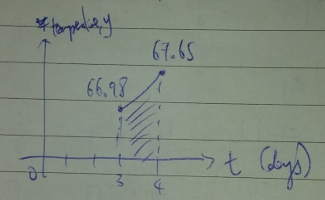
\includegraphics{q1a.jpg}
\end{center}

\begin{tcolorbox}
  \textbf{Q1b)} The number of \emph{cooling degree days} is the sum of reach day of the difference between the average temeperature for that day and $65^{\circ}$. The number is used to estimate the demand for electricity for air conditioning. Draw a second graph of $y$ for the whole 50 days and shade in the region whose area represents the total number of degree days. Write a formula for this total area as the difference between $65 \cdot 50$ and a definite integral. Evaluate the definite integral using the fundamental theorem of calculus. (Alternatively, write the whole quantity as an integral expressing the area between curves as in Lecture 21, and 7.2.)
\end{tcolorbox}

\begin{center}
  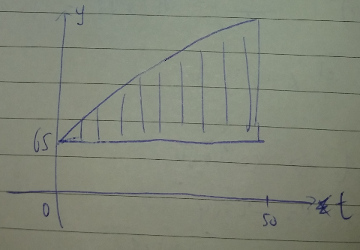
\includegraphics{q1b.jpg}
\end{center}

\begin{align*}
  A &= \int_0^{50} 65 e^{\frac{1}{100}t} dt - 65 \cdot 50 \\
  &= 6500e^{\frac{1}{100}t}\bigg]_0^{50} - 65 \cdot 50 \\
  &= 6500 (e^{\frac{50}{100}} - e^{0}) - \frac{1}{2} \cdot 6500 \\
  &= 6500 (e^{\frac{1}{2}} - \frac{3}{2}) \\
  &\approx 966.688
\end{align*}


\begin{tcolorbox}
  \textbf{Q1c)} (extra credit) Compute the definite integral in part (b) directly by evaluating a lower Riemann sum and taking a limit. Follow the procedure in Problem 5, PS4, but with different scale factors. This rather elaborate calculation shows how much time and effort we save every time we use the fundamental theorem and the change of variable formula in integrals.
\end{tcolorbox}

\begin{center}
  $\int_0^{50} 65 e^{\frac{1}{100}t} dt = 65 \int_0^{50} e^{\frac{1}{100}t} dt$
\end{center}

Since $\frac{d}{dt} e^{\frac{1}{100}t} = \frac{1}{100} e^{\frac{1}{100}t} > 0$, $e^{\frac{1}{100}t}$ is an increasing function. Hence the left Riemann sum is the lower Riemann sum.

Left Riemann sum of $\int_0^{50} e^{\frac{1}{100}t} dt = \sum\limits_{i=0}^{n-1} e^{\frac{1}{100}t_i} \Delta t$ where $\Delta t = \frac{50 - 0}{n} = \frac{50}{n}$

\begin{align*}
  \sum\limits_{i=0}^{n-1} e^{\frac{1}{100}(\frac{50i}{n})} \cdot \frac{50}{n} &= \frac{50}{n} \sum\limits_{i=0}^{n-1} e^{\frac{50i}{100n}} \\
  &= \frac{50}{n} \sum\limits_{i=0}^{n-1} e^{\frac{i}{2n}} \\
  &= \frac{50}{n} \cdot \frac{1(1 - (e^{\frac{1}{2n}})^n)}{1 - e^{\frac{1}{2n}}} \\
  &= \frac{50}{n} \cdot \frac{1 - e^{\frac{1}{2}}}{1 - e ^{\frac{1}{2n}}}
\end{align*}

Use linear approximation for $1 - e^{\frac{1}{2n}}$.

The linear approximation for $e^x = 1 + x$ for $x \approx 0$. Since $\frac{1}{2n} \rightarrow 0$ as $n \rightarrow +\infty$, then $1 - e^{\frac{1}{2n}} \approx 1 - (1 + \frac{1}{2n}) = -\frac{1}{2n}$

Then $n(1 - e^{\frac{1}{2n}}) \approx n \cdot (- \frac{1}{2n}) \approx -\frac{1}{2}$. As $n \rightarrow +\infty$,

\begin{align*}
  \sum\limits_{i=0}^{n-1} e^{\frac{1}{100}(\frac{50i}{n})} \cdot \frac{50}{n} &\approx \lim_{n \rightarrow +\infty} \frac{50}{n} \cdot \frac{1 - e^{\frac{1}{2}}}{1 - e ^{\frac{1}{2n}}} \\
  &\approx \lim_{n \rightarrow +\infty} \frac{50 \cdot (1 - e^{\frac{1}{2}})}{-\frac{1}{2}} \\
  &= -100(1 - e^{\frac{1}{2}}) \\
  &= 100e^{\frac{1}{2}} - 100
\end{align*}

Thus $\int_0^{50} e^{\frac{1}{100}t} dt \approx 100e^{\frac{1}{2}} - 100$ and $65 \int_0^{50} e^{\frac{1}{100}t} dt \approx 65(100e^{\frac{1}{2}} - 100) = 6500e^{\frac{1}{2}} - 6500$


\begin{tcolorbox}
  \textbf{Q2} Consider the function $f(x) = \int_0^{x} cos(t^2) dt$. There is no expression for $f(x)$ in terms of standard elementary functions. It is known as a Fresnel integral, along with the corresponding sine integral. \\
  a) Draw a rough sketch of $cos(t^2)$, showing the first positive and negative zeros. What does the curve look like at $t = 0$? Is the function even or odd?
\end{tcolorbox}

\begin{center}
  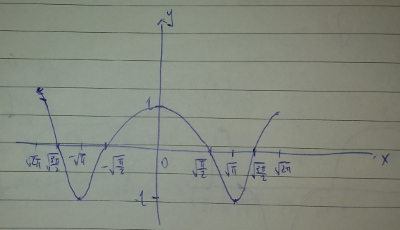
\includegraphics{q2a.jpg}
\end{center}

It is an even function.

\begin{tcolorbox}
  \textbf{Q2b)} List the critical points of $f(x)$ in the entire range $-\infty < x < \infty$. Which critical points are local maxima and which ones are local minima?
\end{tcolorbox}

$\frac{d}{dx}cos(x^2) = 2x(-sin(x^2)) = -2x\ sin(x^2)$

At critical points, $-2x\ sin(x^2) = 0$. Either $x = 0$ or $sin(x^2) = 0$ which implies $x^2 = n\pi$ for some integer $n >= 0$, which means $x = \pm\sqrt{n\pi}$ for some integer $n >= 0$

$\frac{d}{dx}-2x\ sin(x^2) = -2sin(x^2) - 4x^2cos(x^2)$

At $x = 0$, $-2sin(x^2) = 4x^2cos(x^2)$. Either $x = 0$ or $-\frac{1}{2}tan(x^2) = x^2$.

At $x = \pm\sqrt{n\pi}$ for odd $n > 0$, $-4(\pm\sqrt{n\pi})^2cos((\pm\sqrt{n\pi})^2) = -4n\pi cos(n\pi) = -4n\pi (-1) = 4n\pi > 0$. So minimum points are at $\pm\sqrt{n\pi}$ for odd $n > 0$.

At $x = \pm\sqrt{n\pi}$ for even $n$, $-4(\pm\sqrt{n\pi})^2cos((\pm\sqrt{n\pi})^2) = -4n\pi cos(n\pi) = -4n \pi < 0$. So maximum points are at $x = \pm\sqrt{n\pi}$ for even $n > 0$.

When $-4x^2cos(x^2) = 0$, either $x^2 = 0 (x = 0)$ or $cos(x^2) = 0$, which implies $x^2 = \frac{\pi}{2} + n\pi$ for any integer $n >= 0$. That is $\frac{\pi + 2n\pi}{2} = \pi(\frac{2n + 1}{2})$. Hence $x = \pm\sqrt{\pi(\frac{2n + 1}{2})}$ for any integer $n >= 0$.

In summary:

$x = \pm\sqrt{n\pi}$ for odd integer $n > 0$ are minimum points. \\
$x = \pm\sqrt{n\pi}$ for even integer $n > 0$ are maximum points. \\
$x = 0$ is inflection point. \\
$x = \pm\sqrt{\pi(\frac{2n+1}{2})}$ for any integer $n >= 0$ are inflection points.


\end{document}
